%Nicht anfassen, so ist der Dokumentenaufbau
\addtocontents{toc}{\protect\setcounter{tocdepth}{16}}

\addappheadtotoc

\MSonehalfspacing
\appendices
\appendixpage
\appendixtitleoff
%%%%%%%%%%%%%%%%%%%%%%%%%%%%%
%%%Ab hier Inhalt einfügen%%%
%%%%%%%%%%%%%%%%%%%%%%%%%%%%%

\section{Voller und gemeinsamer Bewertungszeitraum}\label{sec:anhang_strukturbruch}
Sämtliche im Ergebnisteil berichteten Vergleiche über Trainingsfenster hinweg wurden auf dem gemeinsamen Zeitraum ab 2010 gerechnet.
Dieser Anhang begründet, warum diese Einschränkung nötig ist, und zeigt, was ohne sie gemessen würde.

Ohne die Einschränkung bewertet jedes Trainingsfenster einen anderen Zeitraum, da der Out-of-Sample-Beginn von März~2000 beim kürzesten auf November~2008 beim längsten Fenster wandert.
Der Lauf mit einem Jahr Training enthält damit das Platzen der Dotcom-Blase, während der Lauf mit zehn Jahren Training erst nach der Finanzkrise beginnt und nur die Erholung abdeckt, wodurch dessen Kennzahlen angehoben werden, ohne dass dies etwas über die Schätzqualität aussagt.
Wie stark der Effekt wiegt, zeigt \hyperref[abb:sharpe_zeitraum]{Abbildung~\ref*{abb:sharpe_zeitraum}}, in der die Sharpe Ratio über die Trainingsfenster einmal über die volle Historie und einmal über den gemeinsamen Zeitraum aufgetragen ist.
Der Sprung beim längsten Fenster tritt links auch beim 1/N-Portfolio auf, obwohl dieses überhaupt keine Schätzung vornimmt, und verschwindet rechts vollständig.
Es handelt sich somit um einen reinen Stichprobeneffekt.

% automatisch erzeugt von paper/abbildungen.py -- nicht von Hand editieren
\begin{figure}[htbp]
  \centering
  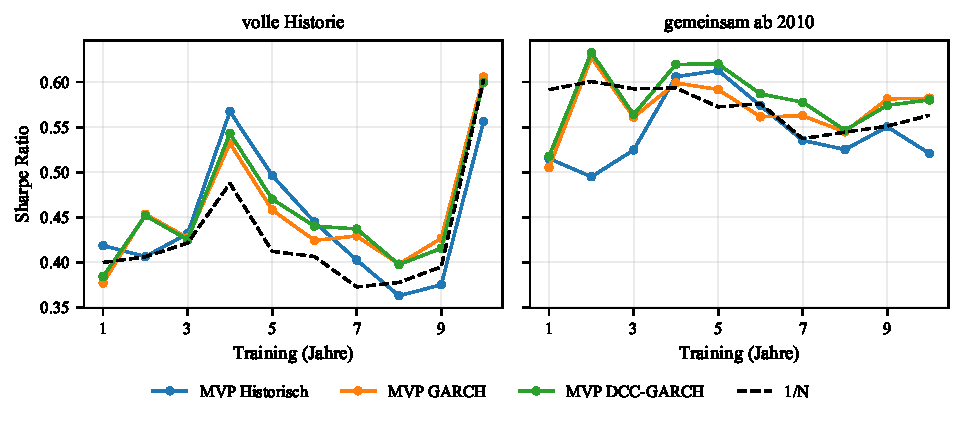
\includegraphics[width=\textwidth]{Abbildungen/abb_sharpe_zeitraum.pdf}
  \caption{Sharpe Ratio über die Trainingsfenster, voller und gemeinsamer Bewertungszeitraum}
  \label{abb:sharpe_zeitraum}
  \begin{minipage}{\linewidth}\vspace{0.4em}\centering\footnotesize
  TRBC, Prognosehorizont 1 Tag, links die volle Historie des jeweiligen Fensters, rechts der für alle Fenster identische Zeitraum ab 01.01.2010.
  \end{minipage}
\end{figure}


\hyperref[tab:strukturbruch_qlike]{Tabelle~\ref*{tab:strukturbruch_qlike}} und \hyperref[tab:strukturbruch_sharpe]{Tabelle~\ref*{tab:strukturbruch_sharpe}} stellen je Trainingsfenster die Kennzahlen über die volle Historie denen über den gemeinsamen Zeitraum ab 2010 gegenüber.
Die erste Tabelle weist neben der mittleren Größe des Anlageuniversums den QLIKE-Verlust der historischen Matrix und der beiden dynamischen Kovarianzschätzer aus, die zweite die Sharpe Ratio des MVP mit allen drei Kovarianzschätzern sowie die des 1/N-Portfolios.
Die 90-\%-Verfügbarkeitsregel lässt die zuletzt hinzugekommenen Sektoren in langen Fenstern erst spät oder gar nicht zu, weshalb die Fensterlänge über die Dimension der Kovarianzmatrix auch das QLIKE-Niveau mitbestimmt.

% automatisch erzeugt von paper/tabellen.py -- nicht von Hand editieren
\begin{table}[htbp]
  \centering
  \footnotesize
  \resizebox{\ifdim\width>\linewidth \linewidth\else \width\fi}{!}{%
  \begin{tabular}{rrrrrrrr}
    \toprule
    Training & $\varnothing\,N$ & \multicolumn{2}{c}{Historisch} & \multicolumn{2}{c}{GARCH} & \multicolumn{2}{c}{DCC-GARCH} \\
    \cmidrule(lr){3-4}\cmidrule(lr){5-6}\cmidrule(lr){7-8}
     & & voll & gem. & voll & gem. & voll & gem. \\
    \midrule
    252 & 20,3 & -161,5 & -176,1 & -161,8 & -175,9 & -162,0 & -176,1 \\
    504 & 19,7 & -159,2 & -171,0 & -160,4 & -171,4 & -160,8 & -171,8 \\
    756 & 19,1 & -156,0 & -165,2 & -157,9 & -166,1 & -158,4 & -166,8 \\
    1008 & 18,5 & -152,8 & -159,7 & -155,4 & -161,1 & -156,1 & -161,9 \\
    1260 & 17,9 & -149,1 & -154,3 & -152,2 & -156,1 & -153,1 & -157,1 \\
    1512 & 17,4 & -146,1 & -150,1 & -149,2 & -151,8 & -150,2 & -152,9 \\
    1764 & 16,9 & -143,0 & -146,0 & -145,9 & -147,7 & -147,0 & -148,8 \\
    2016 & 16,4 & -139,6 & -142,0 & -142,4 & -143,8 & -143,7 & -144,9 \\
    2268 & 16,2 & -138,3 & -140,6 & -141,0 & -142,5 & -142,3 & -143,7 \\
    2520 & 16,2 & -139,1 & -140,0 & -141,3 & -142,0 & -142,7 & -143,3 \\
    \bottomrule
  \end{tabular}
  }
  \caption{QLIKE über vollen und gemeinsamen Bewertungszeitraum (TRBC, $h=1$)}
  \label{tab:strukturbruch_qlike}
  \begin{minipage}{\linewidth}\vspace{0.4em}\centering\footnotesize
  \emph{voll} bezeichnet die volle Historie des jeweiligen Fensters, \emph{gem.} den gemeinsamen Zeitraum ab 01.01.2010. $\varnothing\,N$ ist die mittlere Zahl investierbarer Sektoren im gemeinsamen Zeitraum.
  \end{minipage}
\end{table}


% automatisch erzeugt von paper/tabellen.py -- nicht von Hand editieren
\begin{table}[htbp]
  \centering
  \footnotesize
  \resizebox{\ifdim\width>\linewidth \linewidth\else \width\fi}{!}{%
  \begin{tabular}{rrrrrrrrr}
    \toprule
    Training & \multicolumn{2}{c}{MVP Historisch} & \multicolumn{2}{c}{MVP GARCH} & \multicolumn{2}{c}{MVP DCC-GARCH} & \multicolumn{2}{c}{1/N} \\
    \cmidrule(lr){2-3}\cmidrule(lr){4-5}\cmidrule(lr){6-7}\cmidrule(lr){8-9}
     & voll & gem. & voll & gem. & voll & gem. & voll & gem. \\
    \midrule
    252 & 0,419 & 0,515 & 0,377 & 0,505 & 0,384 & 0,518 & 0,400 & 0,592 \\
    504 & 0,406 & 0,495 & 0,453 & 0,627 & 0,452 & 0,633 & 0,406 & 0,601 \\
    756 & 0,432 & 0,525 & 0,427 & 0,561 & 0,425 & 0,564 & 0,422 & 0,593 \\
    1008 & 0,567 & 0,606 & 0,532 & 0,599 & 0,543 & 0,620 & 0,488 & 0,594 \\
    1260 & 0,496 & 0,613 & 0,458 & 0,592 & 0,470 & 0,620 & 0,412 & 0,573 \\
    1512 & 0,445 & 0,574 & 0,424 & 0,562 & 0,440 & 0,587 & 0,407 & 0,576 \\
    1764 & 0,403 & 0,535 & 0,429 & 0,563 & 0,437 & 0,578 & 0,373 & 0,537 \\
    2016 & 0,363 & 0,525 & 0,398 & 0,545 & 0,398 & 0,547 & 0,378 & 0,545 \\
    2268 & 0,375 & 0,550 & 0,427 & 0,581 & 0,416 & 0,574 & 0,395 & 0,551 \\
    2520 & 0,556 & 0,521 & 0,606 & 0,582 & 0,600 & 0,580 & 0,603 & 0,563 \\
    \bottomrule
  \end{tabular}
  }
  \caption{Sharpe Ratio über vollen und gemeinsamen Bewertungszeitraum (TRBC, $h=1$)}
  \label{tab:strukturbruch_sharpe}
  \begin{minipage}{\linewidth}\vspace{0.4em}\centering\footnotesize
  \emph{voll} bezeichnet die volle Historie des jeweiligen Fensters, \emph{gem.} den gemeinsamen Zeitraum ab 01.01.2010. Ausgewiesen ist die annualisierte Sharpe Ratio.
  \end{minipage}
\end{table}


Wie oft welcher Schätzer über alle 40~Kombinationen vorne liegt, weist \hyperref[tab:bestzaehlung]{Tabelle~\ref*{tab:bestzaehlung}} aus, getrennt nach der Sharpe Ratio je Portfoliomodell und den beiden Verlustmaßen.
Dass die Rangfolge der Schätzer nicht am Basisfall hängt, zeigt sich dort deutlich, da unter beiden Verlustmaßen DCC-GARCH nahezu durchgängig vorne liegt, während ökonomisch bei HRP und ERC die historische Matrix dominiert.

% automatisch erzeugt von paper/tabellen.py -- nicht von Hand editieren
\begin{table}[htbp]
  \centering
  \footnotesize
  \begin{tabular}{lrrr}
    \toprule
    Kennzahl & Historisch & GARCH & DCC-GARCH \\
    \midrule
    Sharpe MVP & 14/40 & 6/40 & 20/40 \\
    Sharpe HRP & 36/40 & 1/40 & 3/40 \\
    Sharpe ERC & 40/40 & 0/40 & 0/40 \\
    \midrule
    QLIKE & 3/40 & 0/40 & 37/40 \\
    Kovarianz-MSE & 0/40 & 1/40 & 39/40 \\
    \midrule
    QLIKE (DCC vs.\ Hist.) & -- & -- & 37/40 \\
    MSE (DCC vs.\ Hist.) & -- & -- & 40/40 \\
    \bottomrule
  \end{tabular}
  \caption{Häufigkeit des besten Kovarianzschätzers je Kennzahl}
  \label{tab:bestzaehlung}
  \begin{minipage}{\linewidth}\vspace{0.4em}\centering\footnotesize
  Alle 40 Kombinationen aus Trainingsfenster und Prognosehorizont, bewertet ab 01.01.2010. In den oberen beiden Blöcken ist ausgewiesen, wie oft der jeweilige Schätzer die höchste Sharpe Ratio beziehungsweise den niedrigsten Verlust liefert; der untere Block zählt zusätzlich direkt, in wie vielen der 40 Läufe DCC-GARCH die historische Matrix schlägt, unabhängig davon, ob GARCH dort noch besser abschneidet.
  \end{minipage}
\end{table}


Zeitlich lokalisieren lässt sich der Bruch über die Teilperioden des Basisfalls in \hyperref[tab:strukturbruch_teilperioden]{Tabelle~\ref*{tab:strukturbruch_teilperioden}}.
Das QLIKE-Niveau springt ab 2022 deutlich nach unten, wobei dieser Sprung exakt mit der Erweiterung des Universums von 17 auf 25~Sektoren im September~2022 zusammenfällt.
Innerhalb der Periode 2022--2026 wächst das Universum anschließend nochmals von 25 auf 27~Sektoren, da zwei erst 2019 gestartete Reihen die 90-\%-Verfügbarkeitsregel im 1008-Tage-Fenster erst 2024 beziehungsweise Ende 2024 erfüllen.
Die Tabellenspanne 17--27 für diese Periode bildet somit beide Schritte ab.
Der MSE zeigt an dieser Stelle keinen vergleichbaren Bruch, folgt dafür aber dem Volatilitätsniveau der Periode und steigt in der Finanzkrise auf mehr als das Siebzigfache des Werts der ruhigen Phase 2003--2007.
Beide Kennzahlen sind über Perioden hinweg somit nur eingeschränkt vergleichbar, wenn auch aus unterschiedlichen Gründen.

% automatisch erzeugt von paper/tabellen.py -- nicht von Hand editieren
\begin{table}[htbp]
  \centering
  \footnotesize
  \resizebox{\ifdim\width>\linewidth \linewidth\else \width\fi}{!}{%
  \begin{tabular}{llrrrrrrrrrr}
    \toprule
    Periode & $N$ & \multicolumn{3}{c}{QLIKE} & \multicolumn{3}{c}{MSE ($\times 10^{-7}$)} & \multicolumn{4}{c}{Sharpe} \\
    \cmidrule(lr){3-5}\cmidrule(lr){6-8}\cmidrule(lr){9-12}
     & & Hist. & GARCH & DCC & Hist. & GARCH & DCC & MVP Hist. & MVP GARCH & MVP DCC & 1/N \\
    \midrule
    2003--2007 & 16--16 & -143,5 & -146,8 & -147,3 & 0,28 & 0,23 & 0,23 & 1,190 & 1,146 & 1,158 & 0,845 \\
    2008--2009 & 16--16 & -119,7 & -130,1 & -131,2 & 21,03 & 16,87 & 16,72 & -0,246 & -0,303 & -0,339 & -0,120 \\
    2010--2019 & 16--17 & -146,1 & -147,2 & -147,8 & 0,79 & 0,61 & 0,60 & 0,886 & 0,969 & 0,982 & 0,719 \\
    2020--2021 & 17--17 & -133,1 & -139,5 & -140,3 & 20,18 & 16,67 & 15,88 & 0,436 & 0,391 & 0,417 & 0,828 \\
    2022--2026 & 17--27 & -205,1 & -204,7 & -205,9 & 1,79 & 1,71 & 1,70 & 0,259 & 0,116 & 0,144 & 0,224 \\
    \bottomrule
  \end{tabular}
  }
  \caption{Teilperioden des Basisfalls: Universum, Prognosequalität und Performance}
  \label{tab:strukturbruch_teilperioden}
  \begin{minipage}{\linewidth}\vspace{0.4em}\centering\footnotesize
  $N$ ist die Spannweite der investierbaren Sektoren; QLIKE-Niveaus sind zwischen Perioden mit unterschiedlichem $N$ nicht vergleichbar.
  \end{minipage}
\end{table}


Aussagekräftig bleibt die Differenz zwischen den Schätzern innerhalb einer Periode, die erheblich variiert.
In der Finanzkrise 2008/09 und im COVID-Zeitraum fällt sie um ein Vielfaches größer aus als in den ruhigen Phasen.
Der Mehrwert der dynamischen Modellierung konzentriert sich damit auf Phasen mit ausgeprägten Volatilitätsschocks, in denen eine statische Matrix dem Risikoniveau am stärksten nachläuft.

Ökonomisch ist die Rangfolge ebenfalls periodenabhängig, da das MVP mit DCC-Kovarianz und ebenso mit GARCH-Kovarianz die historische Variante in der Phase 2010--2019 klar schlägt, in allen übrigen Teilperioden jedoch zurückliegt.
Der Basisfall umfasst die volle Historie ab 2003 und mittelt über gegenläufige Teilperioden, weshalb dort die historische Matrix vorne liegt, während die auf 2010 eingeschränkten Tabellen für das MVP zugunsten von DCC ausfallen.
Beide Rechnungen sind korrekt, messen aber Unterschiedliches, wobei die Unterschiede in beide Richtungen durchgängig insignifikant sind und daher keine starke Aussage zulassen.

\section{Tests auf Sharpe-Differenzen}\label{sec:anhang_sharpetests}
\hyperref[tab:jobson_korkie]{Tabelle~\ref*{tab:jobson_korkie}} weist den Test von \textcite{jobson1981} in der Korrektur von \textcite{memmel2003} für sämtliche paarweisen Vergleiche des Basisfalls aus, sowohl zwischen den Kovarianzschätzern innerhalb eines Portfoliomodells als auch gegenüber dem 1/N-Portfolio.
Kein einziger Vergleich erreicht auch nur das 10-\%-Niveau.

% automatisch erzeugt von paper/tabellen.py -- nicht von Hand editieren
\begin{table}[htbp]
  \centering
  \footnotesize
  \begin{tabular}{lrrr@{}l}
    \toprule
    Vergleich & $\Delta$ Sharpe & $z$-Statistik & \multicolumn{2}{c}{$p$-Wert} \\
    \midrule
    MVP Historisch vs.\ MVP GARCH & 0,0352 & 0,55 & 0,584 &  \\
    MVP Historisch vs.\ MVP DCC-GARCH & 0,0243 & 0,37 & 0,709 &  \\
    MVP GARCH vs.\ MVP DCC-GARCH & -0,0109 & -0,78 & 0,435 &  \\
    HRP Historisch vs.\ HRP GARCH & 0,0063 & 0,30 & 0,764 &  \\
    HRP Historisch vs.\ HRP DCC-GARCH & -0,0041 & -0,18 & 0,859 &  \\
    HRP GARCH vs.\ HRP DCC-GARCH & -0,0104 & -1,23 & 0,220 &  \\
    ERC Historisch vs.\ ERC GARCH & 0,0105 & 0,95 & 0,342 &  \\
    ERC Historisch vs.\ ERC DCC-GARCH & 0,0111 & 0,98 & 0,329 &  \\
    ERC GARCH vs.\ ERC DCC-GARCH & 0,0006 & 0,27 & 0,784 &  \\
    MVP Historisch vs.\ 1/N & 0,0797 & 0,69 & 0,487 &  \\
    MVP GARCH vs.\ 1/N & 0,0445 & 0,41 & 0,681 &  \\
    MVP DCC-GARCH vs.\ 1/N & 0,0554 & 0,51 & 0,611 &  \\
    HRP Historisch vs.\ 1/N & 0,0210 & 0,66 & 0,509 &  \\
    HRP GARCH vs.\ 1/N & 0,0147 & 0,37 & 0,711 &  \\
    HRP DCC-GARCH vs.\ 1/N & 0,0251 & 0,61 & 0,541 &  \\
    ERC Historisch vs.\ 1/N & 0,0132 & 0,85 & 0,395 &  \\
    ERC GARCH vs.\ 1/N & 0,0027 & 0,13 & 0,898 &  \\
    ERC DCC-GARCH vs.\ 1/N & 0,0021 & 0,10 & 0,923 &  \\
    \bottomrule
  \end{tabular}
  \caption{Tests auf Unterschiede der Sharpe Ratios (Basisfall)}
  \label{tab:jobson_korkie}
  \begin{minipage}{\linewidth}\vspace{0.4em}\centering\footnotesize
  Basisfall, bewertet über die volle Historie vom 12.02.2003 bis 09.06.2026. Auf Überschussrenditen über die Fed Funds Rate; $^{***}$, $^{**}$, $^{*}$ = 1-, 5-, 10-\%-Niveau.
  \end{minipage}
\end{table}


\section{Transaktionskosten}\label{sec:anhang_kosten}
\hyperref[tab:transaktionskosten]{Tabelle~\ref*{tab:transaktionskosten}} weist die Sharpe Ratios des Basisfalls nach Abzug proportionaler Transaktionskosten auf das je Rebalancierung umgeschlagene Volumen aus.

% automatisch erzeugt von paper/tabellen.py -- nicht von Hand editieren
\begin{table}[htbp]
  \centering
  \footnotesize
  \begin{tabular}{llrrrrr}
    \toprule
    Modell & Kovarianz & Turnover & 0 Bp. & 5 Bp. & 10 Bp. & 20 Bp. \\
    \midrule
    MVP & Historisch & 0,008 & 0,567 & 0,560 & 0,553 & 0,539 \\
    MVP & GARCH & 0,258 & 0,532 & 0,299 & 0,066 & -0,400 \\
    MVP & DCC-GARCH & 0,255 & 0,543 & 0,310 & 0,077 & -0,388 \\
    \midrule
    HRP & Historisch & 0,012 & 0,509 & 0,499 & 0,490 & 0,472 \\
    HRP & GARCH & 0,072 & 0,502 & 0,447 & 0,391 & 0,279 \\
    HRP & DCC-GARCH & 0,094 & 0,513 & 0,439 & 0,366 & 0,219 \\
    \midrule
    ERC & Historisch & 0,006 & 0,501 & 0,497 & 0,493 & 0,484 \\
    ERC & GARCH & 0,034 & 0,490 & 0,466 & 0,442 & 0,393 \\
    ERC & DCC-GARCH & 0,034 & 0,490 & 0,465 & 0,440 & 0,391 \\
    \midrule
    1/N & -- & 0,006 & 0,488 & 0,484 & 0,480 & 0,472 \\
    \bottomrule
  \end{tabular}
  \caption{Sharpe Ratios nach proportionalen Transaktionskosten (Basisfall)}
  \label{tab:transaktionskosten}
  \begin{minipage}{\linewidth}\vspace{0.4em}\centering\footnotesize
  Sharpe Ratio auf Überschussrenditen über die Fed Funds Rate nach Abzug von $c$ Basispunkten auf das je Rebalancierung umgeschlagene Volumen; die 0-Bp.-Spalte entspricht damit exakt \hyperref[tab:oekonomie_basis]{Tabelle~\ref*{tab:oekonomie_basis}}.
  \end{minipage}
\end{table}


\section{Synthetische Validierung}\label{sec:anhang_synth}
Ob die Modelle korrekt implementiert sind, lässt sich an echten Daten nicht prüfen, da der wahre datengenerierende Prozess unbekannt ist.
Stattdessen werden drei simulierte Datensätze mit jeweils 20~Anlagen und 6.000~Handelstagen verwendet, die dieselbe unbedingte Risikostruktur besitzen (annualisierte Volatilitäten zwischen 15\,\% und 35\,\%, durchschnittliche Korrelation 0,35) und sich ausschließlich in der Dynamik der zweiten Momente unterscheiden.
Der Monte-Carlo-Datensatz enthält unabhängige Ziehungen mit konstanter Kovarianz, in denen die historische Matrix korrekt spezifiziert ist.
Beim GARCH-Datensatz kommt eine GARCH(1,1)-Dynamik je Anlage mit $\alpha = 0{,}08$ und $\beta = 0{,}90$ bei konstanter Korrelation hinzu, während der DCC-Datensatz zusätzlich eine DCC-Rekursion mit $a = 0{,}03$ und $b = 0{,}96$ enthält.
Obwohl die wahre bedingte Kovarianzmatrix hier bekannt wäre, wird die Prognosegüte auch in der Simulation gegen den realisierten Proxy aus \hyperref[eq:proxy]{Gleichung~\ref*{eq:proxy}} gemessen, damit die Ergebnisse mit denen auf den realen Daten vergleichbar sind.

Die Ergebnisse des Basisfalls zeigen \hyperref[tab:synth_basis]{Tabelle~\ref*{tab:synth_basis}} und die DM-Tests in \hyperref[tab:synth_dmw]{Tabelle~\ref*{tab:synth_dmw}}.
Im Monte-Carlo-Fall unterscheiden sich die drei Schätzer praktisch nicht, denn die Verlustdifferenz der dynamischen Schätzer gegenüber der historischen Matrix ist zwar signifikant, in der Höhe aber verschwindend gering.
Im GARCH-Fall schlagen beide dynamischen Schätzer die historische Matrix signifikant, auch in Sharpe Ratio und realisierter Volatilität, unterscheiden sich untereinander aber nicht, da die Korrelation dort konstant ist.
Erst im DCC-Fall ist DCC dem GARCH-Schätzer signifikant überlegen, sodass die Implementierung jeweils genau die Struktur erkennt, die tatsächlich vorhanden ist.

% automatisch erzeugt von paper/tabellen.py -- nicht von Hand editieren
\begin{table}[htbp]
  \centering
  \footnotesize
  \begin{tabular}{llrrrrr}
    \toprule
    Datensatz & Kovarianz & QLIKE & MSE ($\times 10^{-8}$) & Vola (\%) & Sharpe & Turnover \\
    \midrule
    Monte Carlo & Historisch & -154,50 & 7,04 & 11,92 & 0,903 & 0,011 \\
     & GARCH & -154,47 & 7,04 & 11,95 & 0,896 & 0,074 \\
     & DCC-GARCH & -154,47 & 7,04 & 11,95 & 0,896 & 0,075 \\
    \midrule
    GARCH-Sim. & Historisch & -154,23 & 7,84 & 11,37 & 0,756 & 0,010 \\
     & GARCH & -157,25 & 7,57 & 9,85 & 0,854 & 0,154 \\
     & DCC-GARCH & -157,25 & 7,57 & 9,85 & 0,854 & 0,154 \\
    \midrule
    DCC-Sim. & Historisch & -154,13 & 9,86 & 11,93 & 0,561 & 0,011 \\
     & GARCH & -157,02 & 9,19 & 9,62 & 0,773 & 0,160 \\
     & DCC-GARCH & -162,13 & 8,98 & 8,99 & 0,783 & 0,152 \\
    \bottomrule
  \end{tabular}
  \caption{Synthetische Validierung: Basisfall je Datengenerierungsprozess}
  \label{tab:synth_basis}
  \begin{minipage}{\linewidth}\vspace{0.4em}\centering\footnotesize
  20 simulierte Anlagen, Training 1008 Handelstage, Prognosehorizont 1 Tag; Performancekennzahlen für das MVP.
  \end{minipage}
\end{table}


% automatisch erzeugt von paper/tabellen.py -- nicht von Hand editieren
\begin{table}[htbp]
  \centering
  \footnotesize
  \begin{tabular}{lr@{}lrr@{}lrr@{}lr}
    \toprule
    Datensatz & \multicolumn{2}{c}{$\Delta$ G--H} & $t$ & \multicolumn{2}{c}{$\Delta$ D--H} & $t$ & \multicolumn{2}{c}{$\Delta$ D--G} & $t$ \\
    \midrule
    Monte Carlo & 0,029 & $^{***}$ & 6,07 & 0,029 & $^{***}$ & 6,12 & 0,000 &  & 0,32 \\
    GARCH-Sim. & -3,025 & $^{***}$ & -24,69 & -3,024 & $^{***}$ & -24,68 & 0,000 &  & 1,28 \\
    DCC-Sim. & -2,887 & $^{***}$ & -15,64 & -7,998 & $^{***}$ & -35,68 & -5,111 & $^{***}$ & -49,85 \\
    \bottomrule
  \end{tabular}
  \caption{Synthetische Validierung: DM-Tests auf die QLIKE-Differenzen}
  \label{tab:synth_dmw}
  \begin{minipage}{\linewidth}\vspace{0.4em}\centering\footnotesize
  G = GARCH, D = DCC-GARCH, H = historisch; negative Differenzen bedeuten eine bessere Prognose. $^{***}$, $^{**}$, $^{*}$ = 1-, 5-, 10-\%-Niveau.
  \end{minipage}
\end{table}


Wie stabil dieses Bild über die Länge des Trainingsfensters ist, zeigt \hyperref[tab:synth_stabilitaet]{Tabelle~\ref*{tab:synth_stabilitaet}}.
Da das Universum konstant 20~Anlagen umfasst und die Parameter des Prozesses über die gesamte Stichprobe unverändert bleiben, verschiebt sich das Niveau der Prognosekennzahlen kaum, denn das QLIKE-Niveau der historischen Matrix schwankt über alle zehn Fenster um höchstens gut zwei Punkte und das MSE-Niveau bleibt praktisch konstant.
Auch die Rangfolge kehrt sich in keinem Fenster um, da DCC in allen 20~Läufen unter beiden Verlustmaßen besser prognostiziert als die historische Matrix.

Der Vorsprung der dynamischen Schätzer wächst dabei mit der Länge des Trainingsfensters und stabilisiert sich erst bei den längeren Fenstern.
Im DCC-Datensatz steigt der QLIKE-Abstand zwischen DCC und historischer Matrix von 4,1~Punkten bei einem Jahr Training auf 8,5~Punkte bei zehn Jahren, im GARCH-Datensatz von 2,1 auf 2,8~Punkte.
Auch wenn die Modelle also korrekt spezifiziert sind und der Prozess sich nicht verändert, zahlt sich eine breitere Datenbasis für die dynamischen Schätzer weiterhin aus, weil deren zusätzliche Parameter mit mehr Beobachtungen präziser geschätzt werden, während sich das Niveau der historischen Matrix kaum verändert.

% automatisch erzeugt von paper/tabellen.py -- nicht von Hand editieren
\begin{table}[htbp]
  \centering
  \footnotesize
  \resizebox{\ifdim\width>\linewidth \linewidth\else \width\fi}{!}{%
  \begin{tabular}{lrrrrrrrrrrr}
    \toprule
    Datensatz & Training & $N$ & \multicolumn{3}{c}{QLIKE} & \multicolumn{3}{c}{MSE ($\times 10^{-8}$)} & \multicolumn{3}{c}{Sharpe MVP} \\
    \cmidrule(lr){4-6}\cmidrule(lr){7-9}\cmidrule(lr){10-12}
     & & & Hist. & GARCH & DCC & Hist. & GARCH & DCC & Hist. & GARCH & DCC \\
    \midrule
    GARCH-Sim. & 252 & 20 & -154,0 & -156,1 & -156,1 & 7,75 & 7,54 & 7,54 & 0,991 & 0,952 & 0,952 \\
     & 504 & 20 & -154,2 & -156,9 & -156,9 & 7,74 & 7,49 & 7,49 & 0,930 & 0,903 & 0,902 \\
     & 756 & 20 & -154,2 & -157,1 & -157,1 & 7,81 & 7,54 & 7,54 & 0,799 & 0,841 & 0,841 \\
     & 1008 & 20 & -154,2 & -157,3 & -157,2 & 7,84 & 7,57 & 7,57 & 0,756 & 0,854 & 0,854 \\
     & 1260 & 20 & -154,4 & -157,4 & -157,4 & 7,86 & 7,58 & 7,58 & 0,781 & 0,889 & 0,889 \\
     & 1512 & 20 & -155,0 & -157,8 & -157,8 & 6,81 & 6,64 & 6,64 & 0,713 & 0,801 & 0,801 \\
     & 1764 & 20 & -154,8 & -157,6 & -157,6 & 7,00 & 6,84 & 6,84 & 0,706 & 0,826 & 0,826 \\
     & 2016 & 20 & -154,7 & -157,7 & -157,7 & 7,01 & 6,84 & 6,84 & 0,780 & 0,878 & 0,878 \\
     & 2268 & 20 & -154,7 & -157,6 & -157,6 & 7,07 & 6,89 & 6,89 & 0,816 & 0,900 & 0,900 \\
     & 2520 & 20 & -154,7 & -157,5 & -157,5 & 7,00 & 6,84 & 6,84 & 0,744 & 0,823 & 0,823 \\
    \midrule
    DCC-Sim. & 252 & 20 & -156,3 & -158,0 & -160,4 & 9,56 & 8,96 & 8,86 & 0,525 & 0,707 & 0,726 \\
     & 504 & 20 & -155,0 & -157,5 & -161,7 & 9,84 & 9,18 & 9,02 & 0,645 & 0,817 & 0,789 \\
     & 756 & 20 & -154,6 & -157,3 & -162,1 & 9,64 & 8,99 & 8,80 & 0,621 & 0,814 & 0,794 \\
     & 1008 & 20 & -154,1 & -157,0 & -162,1 & 9,86 & 9,19 & 8,98 & 0,561 & 0,774 & 0,783 \\
     & 1260 & 20 & -154,4 & -157,1 & -162,4 & 9,32 & 8,67 & 8,48 & 0,553 & 0,779 & 0,787 \\
     & 1512 & 20 & -154,3 & -157,0 & -162,4 & 9,51 & 8,84 & 8,64 & 0,648 & 0,861 & 0,889 \\
     & 1764 & 20 & -154,1 & -156,9 & -162,3 & 9,72 & 9,03 & 8,82 & 0,681 & 0,807 & 0,868 \\
     & 2016 & 20 & -154,0 & -156,9 & -162,4 & 9,92 & 9,18 & 8,97 & 0,713 & 0,780 & 0,816 \\
     & 2268 & 20 & -153,8 & -156,8 & -162,4 & 10,13 & 9,37 & 9,15 & 0,815 & 0,824 & 0,830 \\
     & 2520 & 20 & -154,0 & -157,0 & -162,5 & 10,04 & 9,28 & 9,06 & 0,977 & 0,982 & 0,964 \\
    \bottomrule
  \end{tabular}
  }
  \caption{Synthetische Validierung: Stabilität über die Trainingsfenster}
  \label{tab:synth_stabilitaet}
  \begin{minipage}{\linewidth}\vspace{0.4em}\centering\footnotesize
  Bewertet über die volle simulierte Stichprobe, da das Universum mit 20 Anlagen konstant ist und die Parameter des Prozesses über die gesamte Reihe unverändert bleiben.
  \end{minipage}
\end{table}


Die ökonomischen Kennzahlen schwanken dagegen auch hier spürbar, obwohl der Prozess vollkommen stabil ist.
Im GARCH-Datensatz erzielt die falsch spezifizierte historische Matrix in den beiden kürzesten Fenstern eine höhere Sharpe Ratio als der DCC-Schätzer.
Im DCC-Datensatz liefert der korrekt spezifizierte DCC-Schätzer in allen zehn Fenstern den besseren QLIKE-Verlust und die niedrigere realisierte Volatilität, beim MVP-Sharpe liegt er jedoch nur in sieben Fenstern vorn und unterliegt in den übrigen dem falsch spezifizierten GARCH-Modell.
Selbst bei bekanntem datengenerierendem Prozess ist die Sharpe Ratio damit zu verrauscht, um Kovarianzschätzer zuverlässig zu ordnen, während die Prognosekennzahlen ein klares und über alle Fenster stabiles Signal liefern.

\begin{landscape}
\section{Dokumentation KI-Nutzung}

\begin{table}[H]
\centering
\small
\renewcommand{\arraystretch}{1.25}
\begin{tabular}{@{}c|>{\raggedright\arraybackslash}p{2.5cm}|>{\raggedright\arraybackslash}p{2.4cm}|>{\raggedright\arraybackslash}p{2.9cm}|>{\raggedright\arraybackslash}p{6.6cm}|>{\raggedright\arraybackslash}p{6.6cm}@{}}
\toprule
\textbf{Nr.} & \textbf{KI-Hilfsmittel} & \textbf{Einsatzform} & \textbf{Betroffene Teile} & \textbf{Beschreibung der KI-Verwendung} & \textbf{Bemerkung} \\
\midrule
1 & Claude & Code & Implementierung & Verwendung von Claude zum Verbessern der Implementierung und Dokumentation & Verwendung zum \enquote{Aufräumen} und Kommentieren des Codes sowie Hilfe bei einzelnen Bugs \\
\hline\addlinespace
2 & Claude \& ChatGPT & Formulierung & Ausformulierung und Stil & Verbesserung der sprachlichen Qualität durch Reduktion von Wortwiederholungen und Korrekturlesen & Hauptsächlich um den Ton einer wissenschaftlichen Arbeit besser zu treffen \\
\hline\addlinespace
3 & Claude & LaTeX & Gesamtes Dokument & Verwendung zur Formatierung in LaTeX & --- \\
\hline\addlinespace
4 & NotebookLM & Analyse von Literatur & Literatur\-auswertung & Verwendung von KI zur Validierung von selbst recherchierten Aussagen aus der Literatur & Literatur wurde selbst recherchiert und selbstständig ausgewertet. KI wurde ausschließlich zur Validierung dieser Aussagen und einer besseren Verknüpfung verschiedener Paper verwendet \\
\bottomrule
\end{tabular}
\caption{Dokumentation der Nutzung von KI-basierten Anwendungen und Werkzeugen}
\label{tab:ki-nutzung}
\end{table}
\end{landscape}
%%%%%%%%%%%%%%%%%%%%%%%%%%%%
%%%%%Ende des Dokuments%%%%%
%%%%%%%%%%%%%%%%%%%%%%%%%%%%
\MSonehalfspacing
\newpage
\restoreapp
